\newpage
\section{Order}
Orders are a new feature in Salespoint 2011. The intention was to prepare the old databaskets for development of web applications and extend them to collaborate with our new inventory, providing the opportunity of individual pricing, final payment and basic log functionality.

\begin{figure}[ht]
	\centering
  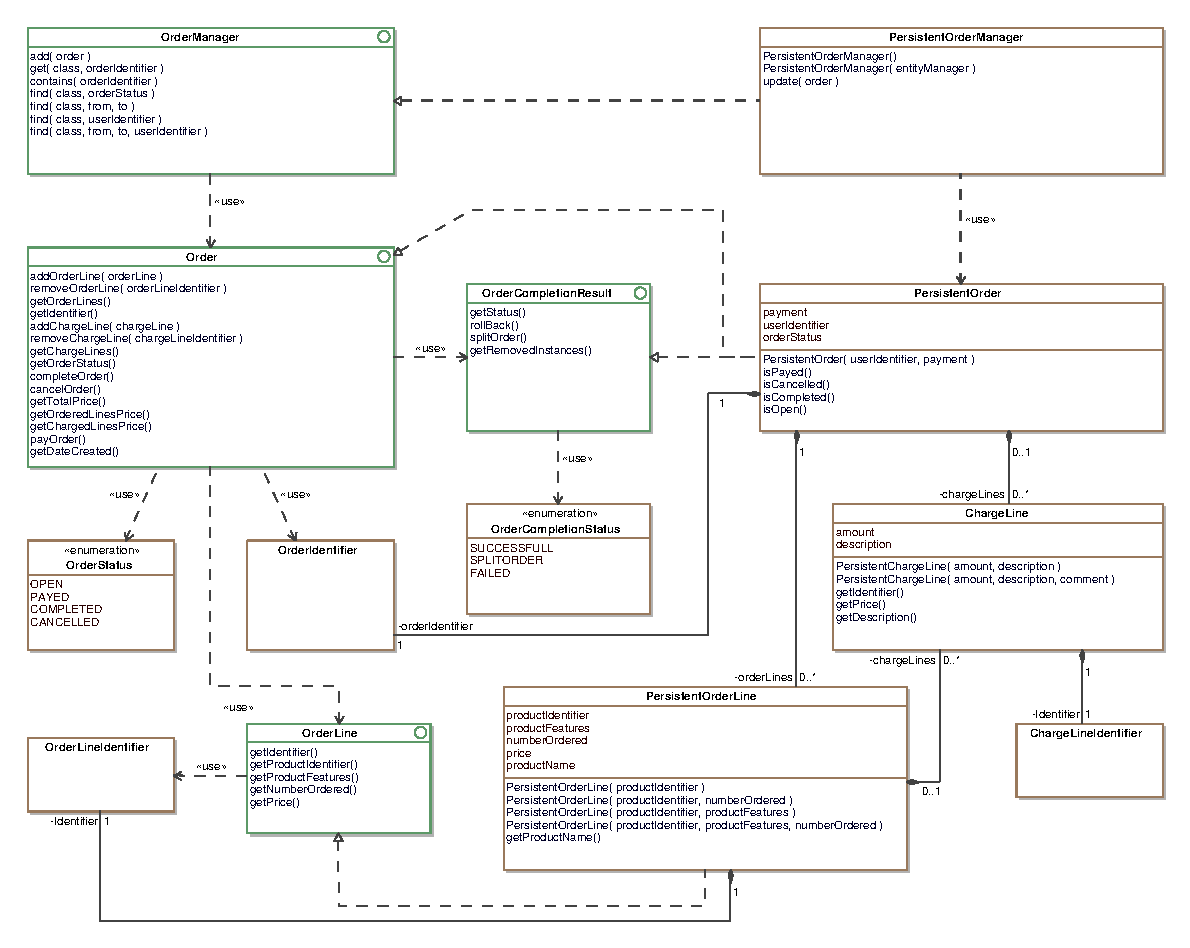
\includegraphics[width=1.0\textwidth]{images/Order_Overview.eps}
	\label{order_overview}
	\caption{Order - Class Overview}
\end{figure}

\subsection{\code{OrderEntry} - The main data structure}
We created the \code{OrderEntry} as main data structure to access the functionality above. An \code{OrderEntry} represents one order and can be imagined as sheet of paper which basically consists of lines representing the ordered products (\code{OrderLine}) and lines that are not bound to a concrete product but which cause charge (\code{ChargeLine}). \code{ChargeLines} make it possible to add individual charge to orders. For example they can be used to define forwarding charges or other special charges produced by this order.
To identify the actor of this order the \code{UserIdentifier} from orderer is also be needed. The \code{SalesChannel} should be used to save information from which channel the order was created (e.g. telephone, internet or mail).

\code{OrderEntrys} are lifecycle-objects. The lifecycle covers four states which are defined by enumeration type \code{OrderEntryStatus}. After all the lifecycle has no restrictions in changing states with one exception: \code{CLOSED} is a final state and it's not possible to change the state of \code{CLOSED} \code{OrderEntrys}. The state machine below shows an example of a frequently practised lifecycle.

\begin{figure}[ht]
	\centering
  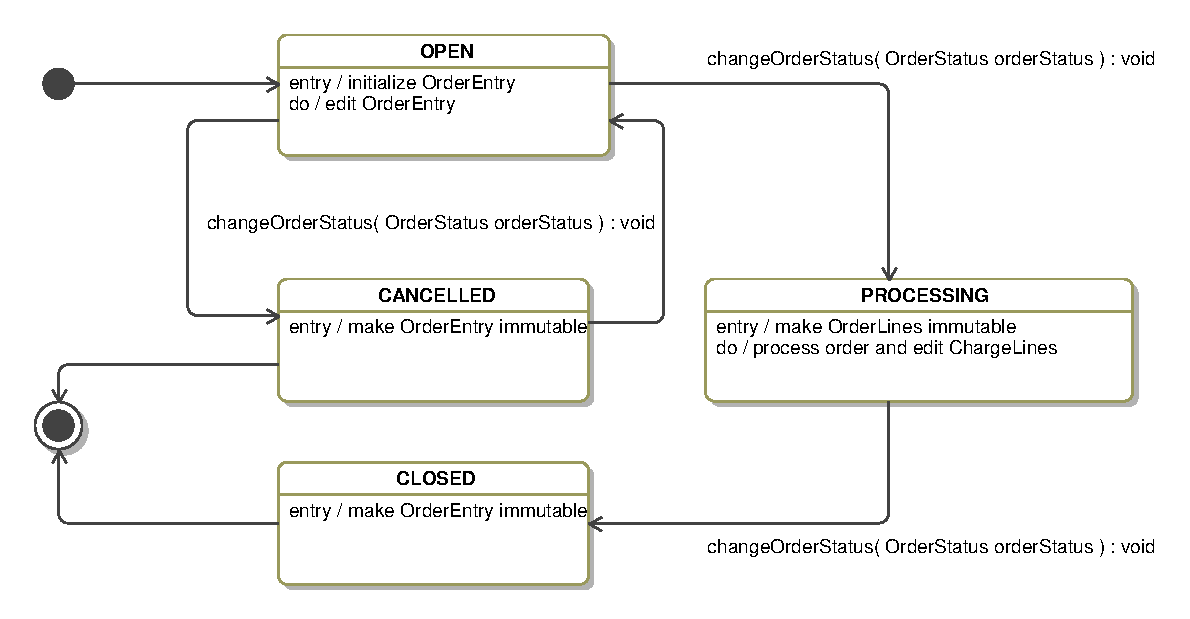
\includegraphics[width=1.0\textwidth]{images/OrderEntryState.eps}
	\label{order_statemachine}
	\caption{Order - Lifecycle}
\end{figure}  

As you can see an OrderEntry can only completely modified in state \code{OPEN}. \code{CANCELLED} and \code{CLOSED} \code{OrderEntrys} are immutable! \code{PROCESSING} \code{OrderEntrys} are basically also immutable but their is still the possibility to modify the \code{ChargeLines} of that \code{OrderEntrys}. 

\subsection{\code{OrderLine} - Representing ordered objects}
An \code{OrderLine} contains all information needed to identify product instances and deal with them. Every \code{OrderLine} is mapped to an \code{Inventory} and contains all \code{Serialnumbers} that are ordered from this \code{Inventory}. Hence an \code{OrderEntry} can contain as far \code{OrderLines} as \code{Inventories} exist. If two or more \code{OrderLines} from same \code{Inventory} will be added to an \code{OrderEntry}, they will be automatically merged into one \code{OrderLine}.

As well as \code{OrderEntrys}, \code{OrderLines} can also contain \code{ChargeLines}. Notice that these \code{ChargeLines} cannot be modified if the \code{OrderLine} is in context of an \code{CANCELLED} or \code{CLOSED} \code{OrderEntry}! 

\subsection{\code{ChargeLine} - Representing additional charge}
A \code{ChargeLine} represents an additional charge for an \code{OrderLine} over and above the \code{OrderLine} value or an extra charge added to an \code{OrderEntry}.

\subsection{\code{OrderLogEntry} - Basic logging structure}
The \code{OrderLogEntry} provides basic logging functionality to show information about actions that where applied to \code{OrderEntrys}. \code{OrderLogEntrys} have a timestamp (\code{dateCreated}) recording when actions are applied. They also have a string that is called \code{action}, which will be filled automatically with action that was procesesed. Finally there is an optional \code{description} string, that can be filled with individual informations.
\code{OrderLogEntries} will be created automatically for all actions that modifiy an \code{OrderEntry}. Therefore all methods that create \code{OrderLogEntries} have versions with or without optional description parameter.

\subsection{\code{OrderManager} - The interface to JPA}
To simplify the management of \code{OrderEntries} we have implemented the \code{PersistentOrderManager}. With \code{PersistentOrderManager} you can persist, update, find and remove \code{OrderEntries}. Contained objects like \code{OrderLines} and \code{ChargeLines} will also be persisted, updated or removed with there \code{OrderEntry} (Cascade).
\code{PersistentOrderManager} are non-Entity classes and cannot be persisted! Multiple \code{OrderManager} in the system working on the same database so it's possible to use seperate \code{PersistentOrderManager} for different tasks, if the functionality is needed. 

